\chapter{CPSolution}
\label{ch:cpsolution}

Aan de hand van een case study van CPSolution, formuleert dit hoofdstuk een antwoord op de tweede deelvraag van het onderzoek:

\begin{center}
	\textit{\textbf{``Hoe wordt de data van het ERP-systeem opgeslagen?''}}
\end{center}

Een korte opfrissing van het begrip ``ERP'' dient als springplank voor een concrete uiteenzetting van het ERP-systeem van 14IT. De daaropvolgende sectie maakt duidelijk dat de evolutie van CPSolution zekere gelijkenissen vertoont met de algemene tendens. 

Hierna wordt de dataopslag van het systeem in kaart gebracht. Een duik onder de motorkap maakt duidelijk hoe wordt omgegaan met data en onder welke structuur dit gebeurt. 

Een laatste sectie over EDI vormt het uitgangspunt voor de \textit{proof of concept}. Het digitaal uitwisselen van data blijft een uitdagende en tijdrovende taak binnen het ERP-verhaal. De huidige gang van zaken kent nog een aantal heikele punten die misschien wel kunnen verholpen worden met de juiste blockchaintoepassingen.


\section{Enterprise resource planning}
\label{sec:enterprise-resource-planning}

Enterprise resource planning (ERP) is de benaming voor software die ontwikkeld werd om een organisatie te ondersteunen bij meerdere bedrijfsprocessen. Dit gaat van processen zoals productie en logistiek tot verkoop, alsook tot boekhouding en HR~\autocite{Shehab2004}. 

Planningsoftware is al langer een vaste waarde in het bedrijfsleven, maar werd oorspronkelijk enkel ingezet voor heel specifieke taken. Zo was er in 1964 al sprake van Material Requirements Planning (MRP). Deze voorouder van ERP stond uitsluitend in voor het inschatten en plannen van productiegoederen. Gaandeweg werd het takenpakket van deze planning- en beheersystemen steeds groter. Daarnaast ontstonden er ook andere \textit{resource planning} systemen voor bedrijfsprocessen zoals shipping, financiële processen, HR en project management~\autocite{Antjon2021}. Om alle onderdelen van een organisatie vanuit een zelfde systeem te ondersteunen en daarbij dubbelwerk te vermijden, werd er gestreefd naar een geïntegreerd systeem: een ERP-systeem~\autocite{Verbeiren2020}. Veelal worden processen onder de vorm van verschillende modules bij elkaar gebracht in eenzelfde pakket.

\begin{figure}[H]
	\centering
	\includegraphics[]{img/cpsolution/erp-diagram.pdf}
	\caption{\label{fig:erp-diagram}ERP als integratie van bedrijfsprocessen~\autocite{Verbeiren2020}}
\end{figure}

\pagebreak

\section{Totstandkoming}
\label{sec:totstandkoming}
In 2014 bracht 14IT het ERP-systeem CPSolution op de markt. Het programma, bestaande uit meerdere modules, is gericht op kmo's en helpt ondertussen een 25-tal klanten bij hun bedrijfsprocessen. CPSolution werd volledig in de taal C\# geprogrammeerd en bestaat uit 36 projecten.

\begin{figure}[H]
	\centering
	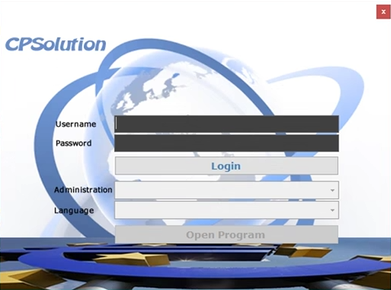
\includegraphics[width=0.6\linewidth]{img/cpsolution/cpsolution.png}
	\caption{\label{fig:cpsolution}Aanmeldpagina van CPSolution}
\end{figure}

CPSolution ontstond niet meteen als een compleet ERP-pakket. In een eerste fase werd het louter ontwikkeld als uitbreiding op een reeds bestaand ordersysteem. Dat gebeurde op vraag van een klant in 2011. Als kaasproducent had de klant nood aan software om orders te plannen op de productielijn. Hun ordersysteem, Unit4 Multivers, bood die \mbox{functionaliteit} echter niet. Daarom werd de vraag gesteld aan 14IT om een oplossing op maat te ontwikkelen. Er werd software geschreven die de orders uit Unit4 Multivers kon ophalen, om vervolgens te plannen op de productielijn. 

Door alsmaar groeiende requirements werd het programma steeds uitgebreid. Zo kon het na verloop van tijd rechtstreeks gebruikt worden voor de opname van orders. Er werden modules toegevoegd om facturen en creditnota's op te maken. Zo was ook de link naar een extern boekhoudsysteem niet meer nodig. Door dergelijke uitbreidingen groeide het programma meer en meer uit tot een autonoom ERP-systeem. In 2014 werd besloten om van hieruit een nieuw softwareproject op te starten onder de naam CPSolution.

\pagebreak

\section{Dataopslag}
\label{sec:dataopslag}

\subsection{Type databank}
\label{sub:type-databank}

De data van het ERP-systeem wordt opgeslagen in een relationele databank van Microsoft SQL Server. De gebruikte editie is afhankelijk van de grootte en de noden van de klant. Voor kleine bedrijven volstaat een Express-editie soms al. Voor klanten zoals Lumap, die maandelijks honderden facturen te verwerken krijgen, is een Enterprise editie aangewezen. Onderstaande tabel is een greep uit de Microsoft documentatie om een beeld te geven van deze edities.

\begin{table}[H]
	\centering
	\begin{tabular}{@{}lccc@{}}
		\cmidrule(l){2-4}
		Maximum ...                                                                           & \textbf{Express}                                                         & \textbf{Standard}                                                          & \textbf{Enterprise} \\ \midrule
		\begin{tabular}[c]{@{}l@{}}compute capacity \\ used by a single instance\end{tabular} & \begin{tabular}[c]{@{}c@{}}lesser of 1 socket \\ or 4 cores\end{tabular} & \begin{tabular}[c]{@{}c@{}}lesser of 4 sockets\\  or 24 cores\end{tabular} & OS maximum          \\ \midrule
		\begin{tabular}[c]{@{}l@{}}memory for buffer \\ pool per instance\end{tabular}        & 1410 MB                                                                  & 128 GB                                                                     & OS maximum          \\ \midrule
		\begin{tabular}[c]{@{}l@{}}memory-optimized \\ data size per database\end{tabular}    & 352 MB                                                                   & 32 GB                                                                      & unlimited           \\ \midrule
		relational database size                                                              & 10 GB                                                                    & 524 PB                                                                     & 524 PB              \\ \bottomrule
	\end{tabular}
	\caption{\label{tab:sql-server-edities}Vergelijking van Microsoft SQL Server 2019 edities}
\end{table}


\subsection{Hosting}
\label{sub:hosting}

Naast de editie van de databank is ook de hosting van belang. Voor het ontwikkelen van CPSolution laat 14IT een databank hosten door Combell. In gebruik hebben klanten drie keuzes voor de fysieke opslag van deze databank:

\begin{itemize}
	\item \textbf{On-premises:} De databank wordt opgeslagen op een toestel in het intern netwerk van de klant. Indien nodig installeert 14IT hiervoor de nodige hardware. Deze optie vraagt dus een zekere investering van de klant, maar heeft als voordeel dat de data heel snel raadpleegbaar is.
	\item \textbf{Combell-hosting:} Er wordt beroep gedaan op een van de databasepaketten van Combell. Aangezien de software lokaal bij de klant geïnstalleerd wordt, dient men rekening te houden met een zekere latentie.
	\item \textbf{CPSolution on Cloud:} De databank en software worden opgeslagen op een fysiek toestel van 14IT dat instaat als server. Om de toepassing te delen met de klant bestaan twee mogelijkheden. Ofwel opteert de klant voor een published application. De klant zal lokaal een applicatie kunnen openen. Hoewel het lijkt alsof de applicatie lokaal draait, wordt er achterliggend eigenlijk een sessie op de server gestart. Enkele klanten maken gebruik van remote desktop om zo te interageren met het toestel. Dat is de tweede optie.
\end{itemize}

\subsection{Datamodel}
\label{sub:datamodel}

De databank van CPSolution is opgebouwd volgens een relationeel model. Het model begon kleinschalig, maar groeide uit tot een enorm netwerk van tabellen. Dat gebeurde naargelang er nieuwe requirements kwamen van klanten. Momenteel is het datamodel zodanig uitgebreid dat het vrijwel niet op papier voor te stellen valt. Onderstaande afbeelding is slechts een deel van het ERD. Dat geeft al een idee van de omvang van de databank.

\begin{figure}[H]
	\centering
	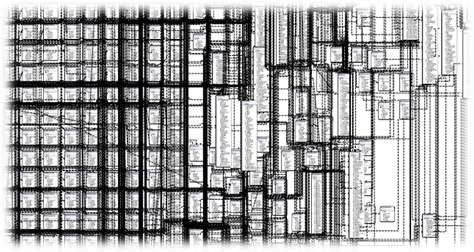
\includegraphics[width=0.6\linewidth]{img/cpsolution/cpsolution-dbml.png}
	\caption{\label{fig:cpsolution-dbml}Blik op het datamodel van CPSolution}
\end{figure}


Om orde aan te brengen in het enorme aantal tabellen, werkt 14IT met een vaste naamgeving.
Tabellen die conceptueel rond eenzelfde thema draaien, worden voorafgegaan door eenzelfde afkorting. Op die manier worden de tabellen onderverdeeld in subcategorieën die van elkaar gescheiden worden met een onderstrepingsteken. Alle tabellen inzake producten worden bijvoorbeeld voorafgegaan door de aanduiding \verb*|PROD_|. Bepaalde subgroepen van de producttabellen kunnen nog verder gegroepeerd worden. Tabellen die beginnen met \verb*|CPS_PROD_PA_| zijn daar een voorbeeld van. Ze betreffen de ``PurchaseAgreements'' van producten. 

\begin{figure}[H]
	\centering
	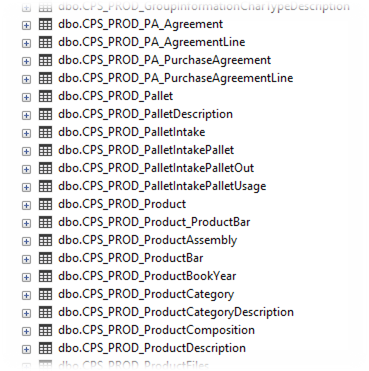
\includegraphics[width=0.45\linewidth]{img/cpsolution/naamgeving-tabellen.png}
	\caption{\label{fig:naamgeving-tabellen}Naamgeving van tabellen}
\end{figure}

De databank van CPSolution kent een heel aantal prefixen. Deze hangen vaak samen met een bepaalde module. Aangezien een lijst met modules\footnote{Zie Bijlage \ref{ch:modules-van-cpsolution} -- \nameref{ch:modules-van-cpsolution}} iets bevattelijker is, is het niet nodig om al deze prefixen ook op te lijsten.

Enkele bijzondere tabellen zijn die met prefix:
\begin{itemize}
	\item \verb*|IMP_|: Deze tabellen dienen als tussenstap om data uit Excel-bestanden van een klant te importeren in de databank. In deze tussenstap kan gecontroleerd worden of de data compleet en consistent is. Daarna kan men op basis van deze tabel kiezen welke rijen al dan niet geïmporteerd moeten worden. Dan gaat die data van de \verb*|IMP|-tabel naar zijn \verb*|CPS|-equivalent.
	\item \verb*|BCK_|: De tabellen die gebruikt worden om back-ups van de data te voorzien.
	\item \verb*|ERR_|: Een tabel die errors en logs van het systeem bijhoudt.
	\item \verb*|LOGS_|: Lijst van logins met gebruikersnaam en tijdstip.
	\item \verb*|X_|: Wanneer klanten specifieke databehoeften hebben, is er soms nood aan een tabel die enkel voor die klant gebruikt zal worden. Die krijgen deze aanduiding.
	\item \verb*|MON_|: 14IT kan indien gewenst allerlei processen bij de klant monitoren. Zo kan men bijvoorbeeld nagaan of er een probleem is met de automatische back-ups. Hiervoor wordt op geregelde tijdstippen data opgeslagen in de \verb*|MON|-tabellen. 
\end{itemize}

Tabellen met het achtervoegsel ``Description'' houden de vertalingen bij van een specifieke tabel. Zo worden de vertalingen voor de records in \verb*|CPS\_PROD\_Product| bijgehouden in de tabel \verb*|CPS_PROD_ProductDescription|. Standaard worden de talen Engels, Frans en Nederlands voorzien. Klanten kunnen echter ook een extra module aanvragen om zelf extra vertalingen te voorzien in een andere taal zoals het Pools.

Wanneer een klant een nieuwe requirement stelt voor het ERP-systeem, wordt vanuit ontwikkeling steeds bekeken of het praktijkprobleem van dat bedrijf kan veralgemeend worden naar een module die voor meerdere klanten interessant is. Zulke uitbreidingen of wijzigingen vereisen soms een zekere datarefactoring. Het ontwerp van de databank wordt dan aangepast, met als doel een zo generiek mogelijk systeem te ondersteunen. 


\section{Electronic data interchange}
\label{sec:electronic-data-interchange}
Sinds de digitale revolutie is het gangbaar geworden om bedrijfsdocumenten zoals facturen, orders en rekeningen elektronisch uit te wisselen. Dit gegeven kreeg de algemene term ``electronic data interchange'' (EDI) toegeschreven. 
EDI biedt als voordeel dat het ontvangende bedrijf het document efficiënter kan opnemen in een eigen digitaal systeem~\autocite{Ford2007}. Een fysiek document, daarentegen, vereist daarvoor manuele ingave of geavanceerde technieken zoals OCR\footnote{Optical character recognition software kan gebruikt worden om tekst te extraheren uit een afbeelding.}. Desondanks blijven ook deze papieren varianten een vaste waarde in het bedrijfsleven.

\subsection{Moeilijkheden}

Het hele EDI-gebeuren vereist dat de interne systemen van onderhandelende partijen op elkaar afgestemd zijn. Voor software-ontwikkelaars is dit geen evidente opdracht. 

\subsubsection{Aaneenschakeling}
Een deel van dit probleem probeerde men te vereenvoudigen door vaste EDI-standaarden af te spreken. Ondernemingen kunnen dan de nodige ``vertalingen'' voorzien van hun data naar het gedeelde formaat, in plaats van een rechtstreekse omzetting te moeten maken naar externe systemen. Dergelijke omzettingen, veroorzaken weinig problemen indien het een enkele overschakeling betreft~\autocite{Damsgaard2000}. Binnen de context van een \textit{supply chain}, waar factuurdata doorheen verschillende ondernemingen moeten gaan, kan een veelvoud van ``vertalingen'' er echter voor zorgen dat de benodigde, correcte data verloren gaan. Als analogie kan men dit probleem vergelijken met het spelletje ``Chinees gefluister''\footnote{Chinees gefluister is de naam van een spelletje waarin kinderen op een rij staan, met als doel een boodschap van persoon tot persoon door te fluisteren. Vaak probeert men met dit spelletje de kinderen te laten ondervinden dat de boodschap drastisch veranderd kan zijn, op het moment dat het bij de laatste schakel aankomt.}. In een ideaal scenario zou de oorsponkelijke data van elke stap in de schakel steeds beschikbaar moeten blijven.


\subsubsection{Confidentialiteit}
Daarnaast is het ook belangrijk dat de data de juiste ontvanger bereikt. Data over de onderhandelingen tussen twee ondernemingen moeten niet openbaar zijn, maar moeten tegelijk wel steeds op een vlotte manier raadpleegbaar zijn voor beide partijen.

\subsubsection{Verifieerbaarheid}

In de andere richting moet de ontvanger ook kunnen verifiëren dat de data van de juiste partij afkomstig is. In de praktijk gaat dit soms zelfs nog gepaard met manuele checks op basis van papieren facturen. Daarnaast moet ook nog de digitale versie van de factuur nagekeken worden. Dat zorgt voor heel wat dubbelwerk. 


\subsection{As is}
CPSolution staat niet rechtstreeks in contact met andere systemen om aan EDI te doen. Hiervoor wordt beroep gedaan op de services van Basware. Bestanden zoals orders en facturen worden als een gestructureerde XML naar BasWare gestuurd. Zij vormen het om naar het juiste EDI formaat en sturen dit door naar de ontvanger. Gezien deze uitbesteding en de moeilijkheden die gepaard gaan met EDI, is het interessant om een alternatief te zoeken voor dit aspect van CPSolution.




